\section{Case Study}
% PZ: I think the two sentences below should in 'Methods' section.
%We have developed an open-source tool dReach using OCaml to perform $\delta$-complete reachability
%analysis for hybrid systems \cite{dreach}. dReach is built upon our SMT solver dReal \citep{dreal}
%that implements a $\delta$-complete decision procedure.

To exemplify different aspects of our parameter synthesis framework, we carried out a case study on
a model of the cardiac cell electrical dynamics. All the experiments reported below were done
using a machine with two Intel Xeon E5-2650 2.00GHz processors and 64GB RAM. The precision $\delta$
was set to $0.001$.

\begin{figure}[t]
\centering
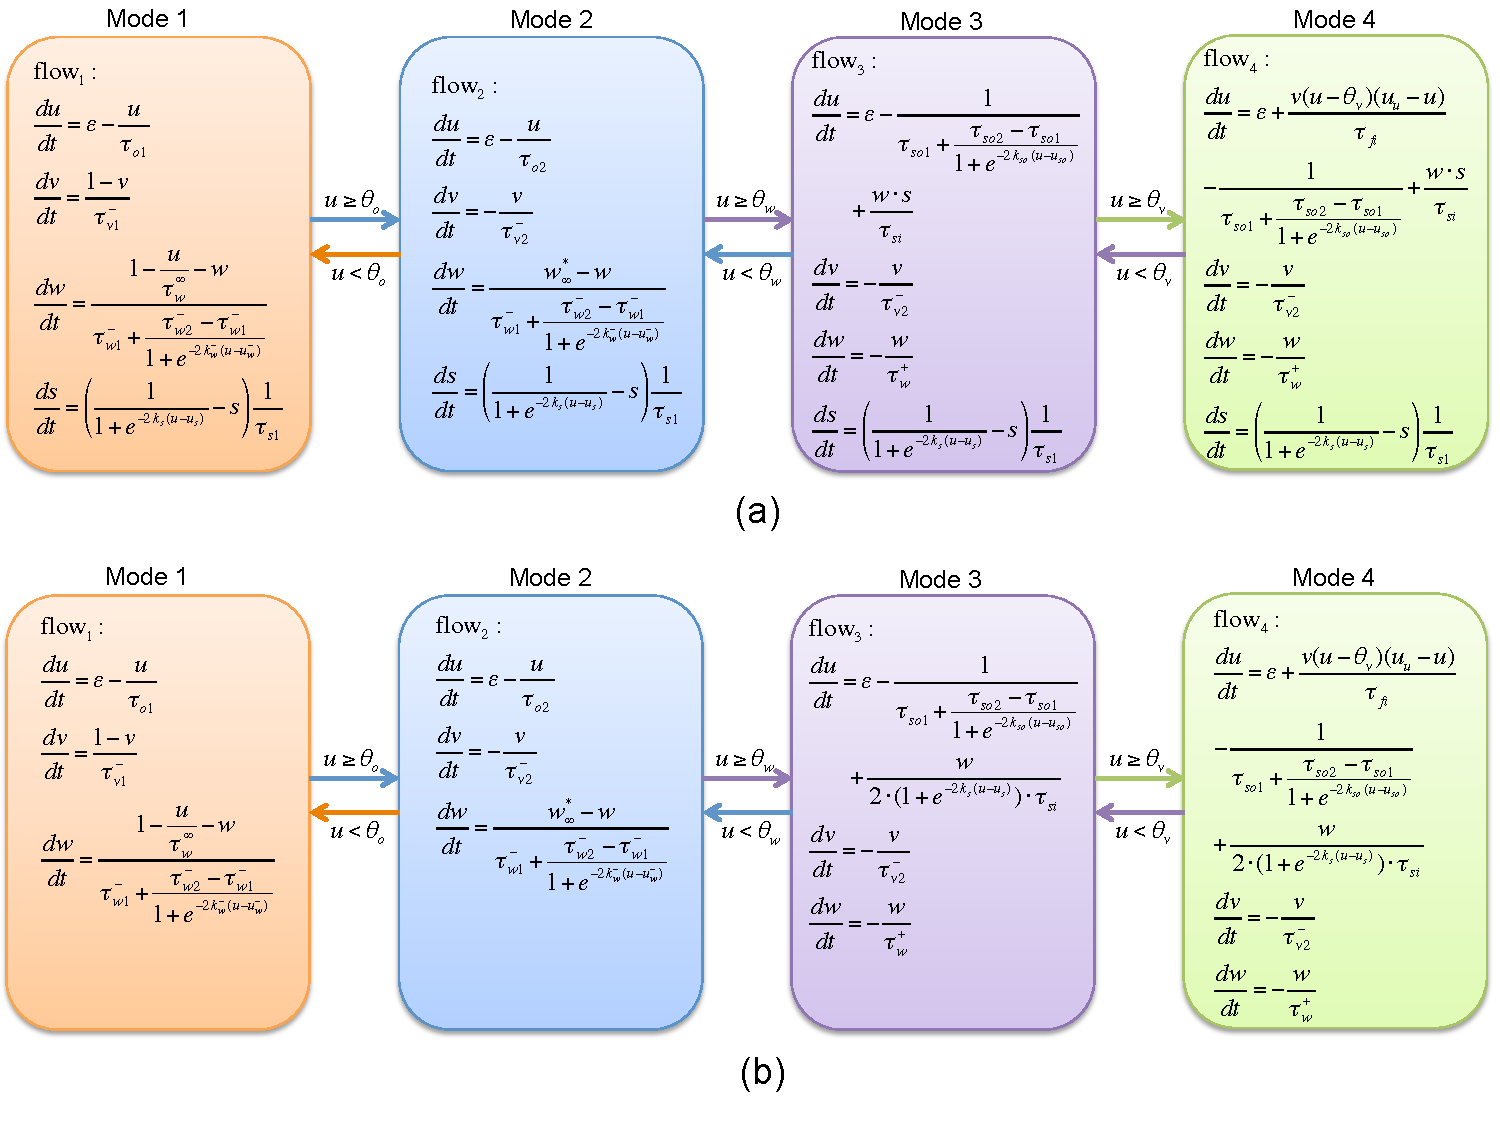
\includegraphics[scale=0.5]{fig-cardiac-new}
\caption{Hybrid models of cardiac cells. (a) BCF model. (b) FK model.}
\label{model}
 %\vspace{-0.7cm}
\end{figure}

\subsection{Hybrid models of cardiac cells}
The heart rhythm is enabled by the electrical activity of cardiac muscle cells, which make up the atria and ventricles. The electrical dynamics of cardiac cells is governed by the organized opening and closing of ion channel gates on the cell membrane. Improper functioning of the cardiac cell ionic channels can cause the cells to lose excitability, which disorders electric wave propagation and leads to cardiac abnormalities such as ventricular \textit{tachycardia} or \textit{fibrillation}. In order to understand the mechanisms of cardiac disorders,
hybrid automata models have been recently developed, including the Fenton-Karma (FK) model \cite{fenton98} and the Bueno-Cherry-Fenton (BCF) model \cite{orovio08}.

\paragraph{BCF Model.}
In this model, the change of cells transmembrane potential $u$, in response to an external stimulus $\epsilon$ from neighboring cells, is regulated by a fast ion channel gate $v$ and two slow gates $w$ and $s$.
Figure \ref{model}(a) shows the four modes associated with the BCF model. In Mode $1$, gates $v$ and $w$ are open and gate $s$ is closed. The transmembrane potassium current causes the decay of $u$. The cell is resting and waiting for stimulation. We assume an external stimulus $\epsilon$ equal to $1$ that lasts for $1$ millisecond. The stimulation causes $u$ to increase, which may trigger $\jump_{1 \rightarrow 2}: u \geq \theta_o$. When this jump takes place, the system switches to Mode 2 and $v$ starts closing, and the decay rate of $u$ changes. The system will jump to Mode 3 if $u \geq \theta_w$. In Mode 3, $w$ is also closing; $u$ is governed by the potassium current and the calcium current. When $u \geq \theta_v$, Mode 4 can be reached, which signals a successful action potential (AP) initiation. In Mode 4, $u$ reaches its peak due to the fast opening of the sodium channel. The cardiac muscle contracts and $u$ starts decreasing.

\paragraph{FK Model.}
As shown in Figure \ref{model}(b), this model comprises the same four modes and equations of the BCF model, except that the current change induced by gate $s$ is reduced to an explicit term which is integrated in the right-hand side of $du/dt$. Similarly to the BCF model, an AP can be successfully initiated when Mode 4 is reached.

\vspace{1ex}
We specified both the BCF and the FK models using dReach's modeling language. Starting from the state ($u = 0$, $v = 1$, $w = 1$, $s = 0$) in Mode 1, we checked whether Mode 4 is reachable using the parameter values presented in \cite{orovio08}. This was true (\ie, dReach returned $\delta$-$\mathsf{sat}$) for both models.
The simulation of a few witness trajectories are shown in Figure \ref{trace} (the stimulus $\epsilon$ was reset every $500$ milliseconds).


\begin{figure}[thb]
\centering
\subfigure[]{
  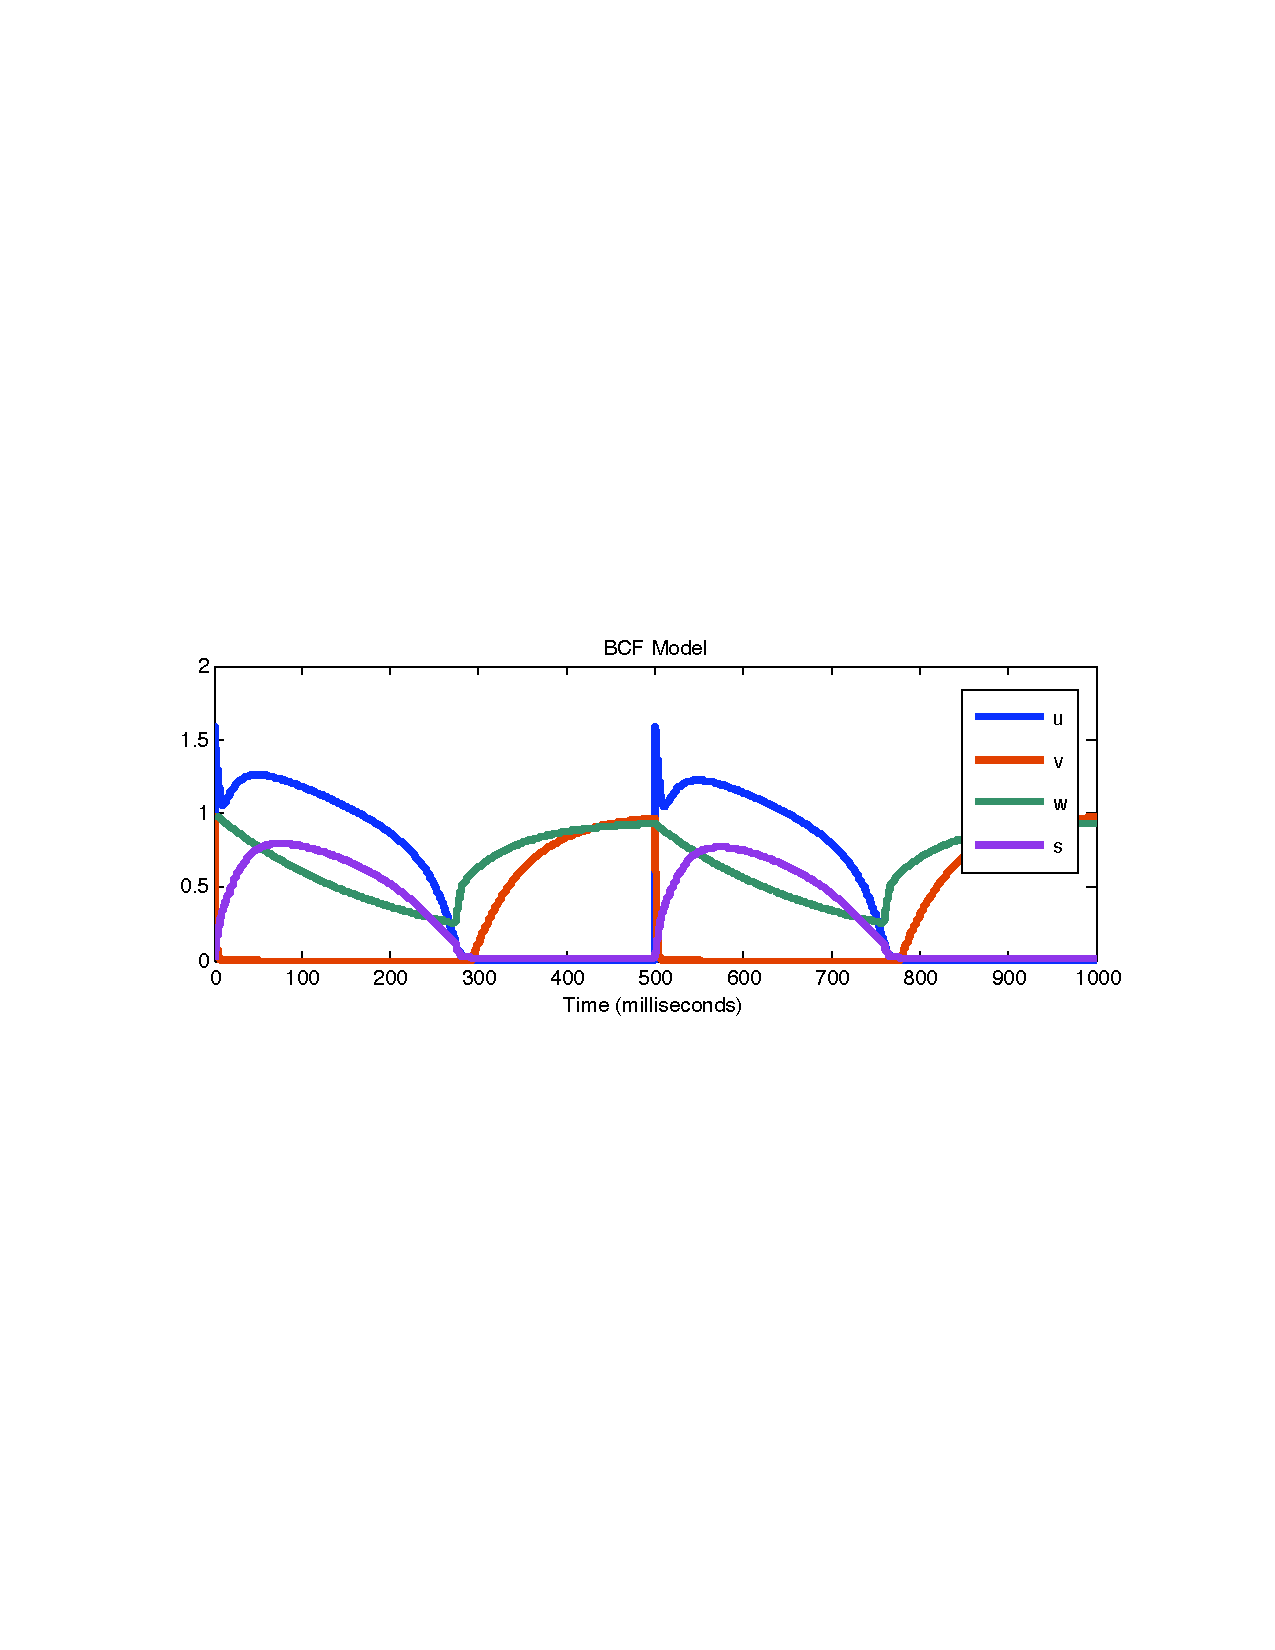
\includegraphics[width=8cm]{fig-bcf}
}
\subfigure[]{
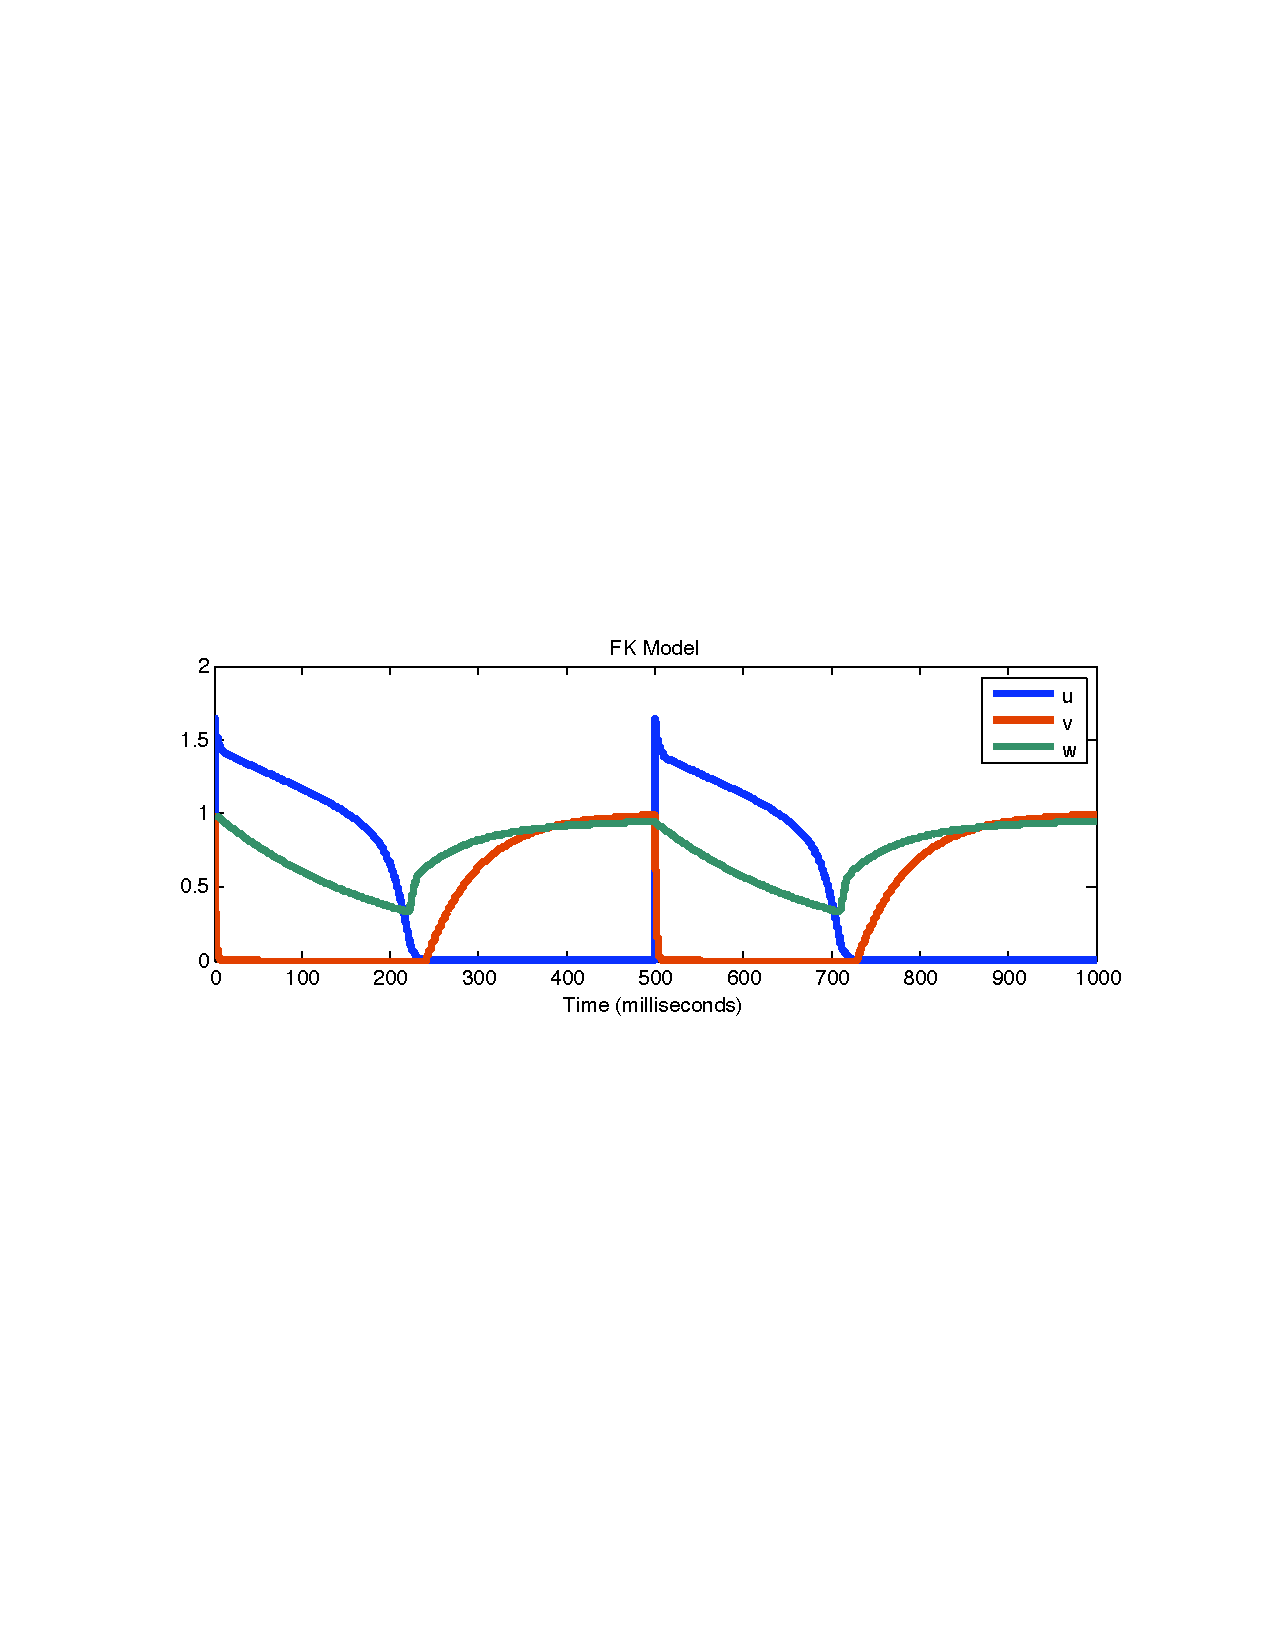
\includegraphics[width=8cm]{fig-fk}
}
\caption{The simulated time profile of BCF and FK.}
\label{trace}
 %\vspace{-0.7cm}
\end{figure}


\subsection{Model falsification}
Both the BCF and the FK models were able to reproduce essential characteristics (\eg, steady-state action potential duration) observed in human ventricular cells \cite{fenton98,orovio08}. However, ventricular cells comprise three cell types, which possess different dynamical characteristics. For instance, Figure \ref{ap} shows that time courses of APs for epicardial and endocardial human ventricular cells have different morphologies \cite{nabauer96}. The important \textit{spike-and-dome} AP morphology can only be observed in epicardial cells but not endocardial cells. Hence, in a model-based study, one needs to identify cell-type-specific parameters to take account into cellular heterogeneity. The feasibility of this task will depend on the model of choice, as for certain models it would be impossible to reproduce a dynamical behavior no matter which parameter values are used. Here we illustrate that such models can be ruled out efficiently using our $\delta$-decision based parameter synthesis framework.

\paragraph{Robustness.}
To ensure proper functioning of cardiac cells in noisy environments, an important property of the system is to filter out insignificant stimulation. Thus, we expected to see that AP could not be initiated for small $\epsilon$. Starting from the state ($u = 0$, $v = 1$, $w = 1$, $s = 0$, $\epsilon \in [0.0,0.25]$) in Mode 1, we checked the reachability of Mode 4. The $\mathsf{unsat}$ answer was returned by dReach for both the BCF and FK
model, showing that the models are robust to stimulation amplitude.

\begin{figure}[th]
\centering
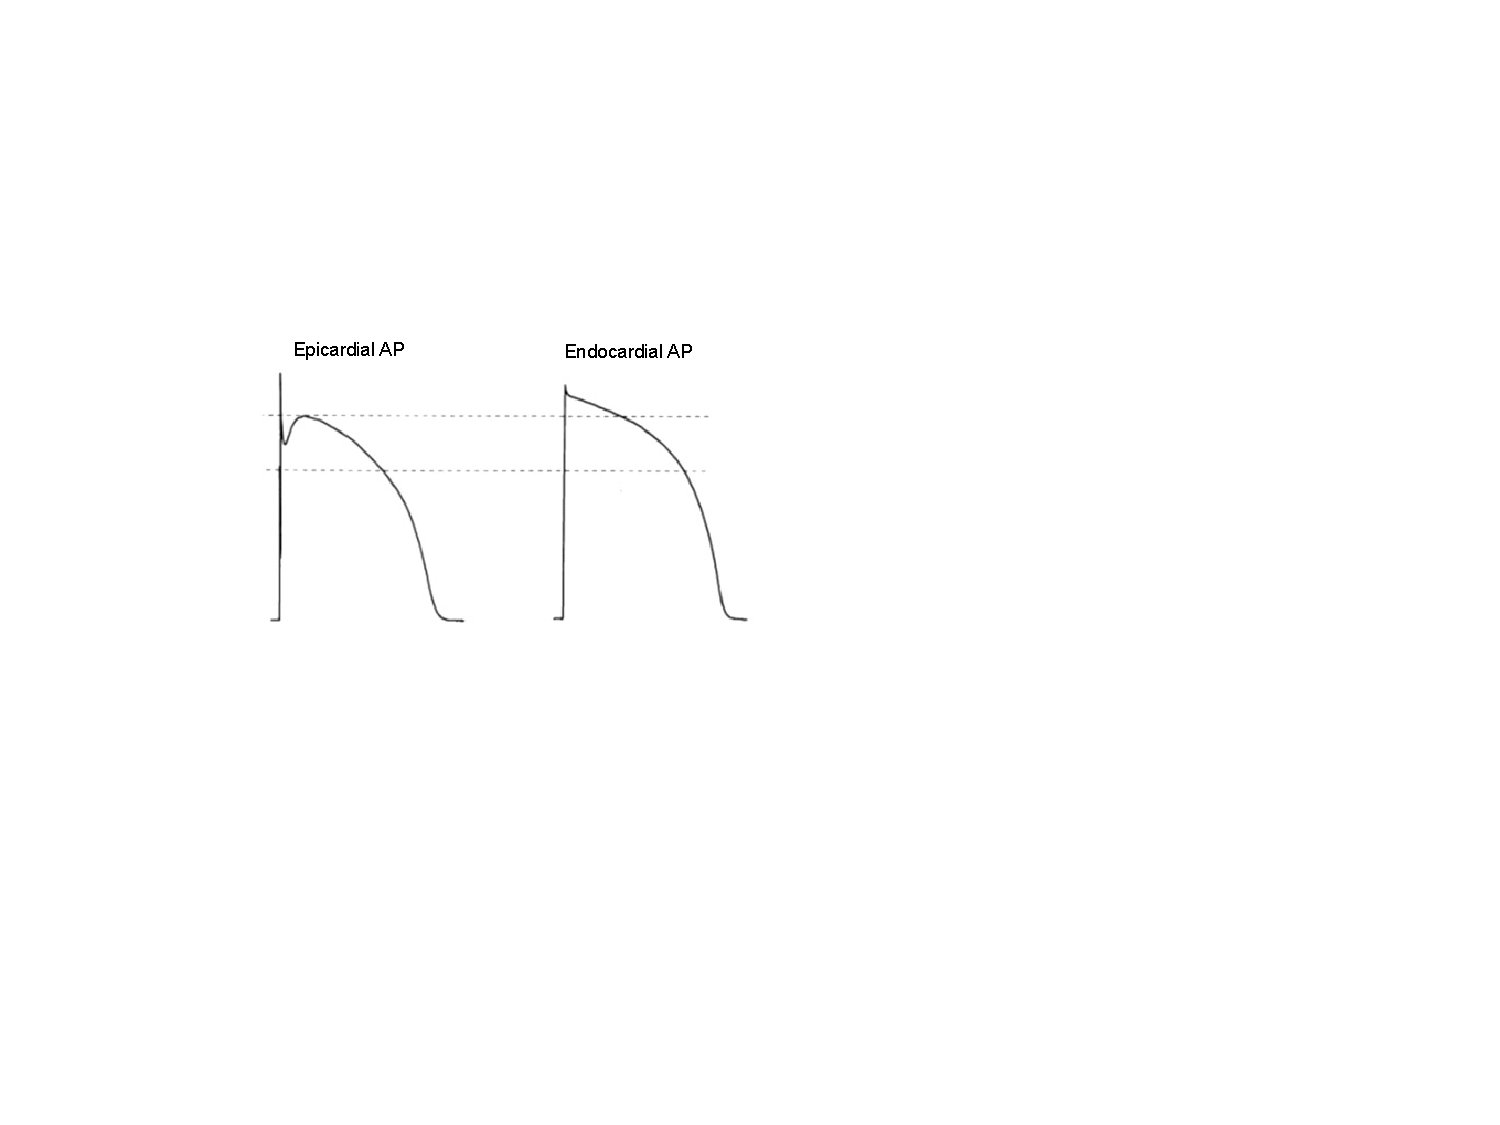
\includegraphics[scale=0.8]{fig-ap}
\caption{Experimental AP morphology \cite{nabauer96}.}
\label{ap}
 %\vspace{-0.7cm}
\end{figure}

\paragraph{AP morphology.}
Next we tested whether the models can reproduce the spike-and-dome AP morphology of epicardial cells. We introduced two auxiliary modes (Mode 5 and 6). The system will jump from Mode 4 to Mode 5 if $\text{\em time} \le 10$, and will jump from Mode 5 to Mode 6 if $\text{\em time} \le 30$. In Modes 5 and 6, we enforced invariants $1.0 \le u \le 1.15$ and $1.18 \le u \le 2.0$, respectively, to depict the spike-and-dome morphology observed experimentally \cite{nabauer96}. We then checked reachability of Mode 6, starting from Mode 1 in state ($u = 0$, $v = 1$, $w = 1$, $s = 0$, $\epsilon \in [0.9,1.1]$, $\tau_{si} \in [1,2]$, $u_s \in [0.5,2]$),
where $\tau_{si}$ and $u_s$ are two model parameters that govern the dynamics of $u$ and $s$ in
Mode 3 and 4 (see Figure \ref{model}).
The $\delta$-$\mathsf{sat}$ answer
was returned for BCF, while $\mathsf{unsat}$ was returned for FK, indicating that the FK model cannot reproduce spike-and-dome shapes using reasonable parameter values. Hence, FK is not suitable to study the dynamics of epicardial cells.

We remark that any $\mathsf{unsat}$ answer is guaranteed to be correct. This effectively
means that we proved that the FK model cannot reach Mode 6 for {\em any} starting state in the
rectangle ($u = 0$, $v = 1$, $w = 1$, $s = 0$, $\epsilon \in [0.9,1.1]$, $\tau_{si} \in [1,2]$,
$u_s \in [0.5,2]$). Sampling-based approaches cannot have the same level of certainty, while other
approaches cannot handle the complexity of the flows in the model.


\subsection{Parameter identification for cardiac disorders}

When the system cannot reach Mode 4, the cardiac cell loses excitability, which might lead to tachycardia or fibrillation. Starting with Mode 1, our task was to identify parameter ranges for which the system will never go into Mode 4. In what follows, we focused our study on the BCF model.
Grosu {\em et al.}~\cite{grosu11} have tackled this parameter identification problem by linearizing the BCF model into a piecewise-multiaffine system (referred as MHA). With this simplification, parameter ranges could be identified using the Rovergene tool \cite{rovergene}. However, the BCF and MHA models have different sets of parameters. Here we aimed at identifying disease-related ranges of the {\em original} BCF parameters. It can be derived from the model equations that $\tau_{o1}$ and $\tau_{o2}$ govern the dynamics of $u$ in Mode 1 and Mode 2 respectively, and hence determine whether $\jump_{1\rightarrow 2}$ and  $\jump_{2\rightarrow 3}$ can be triggered. For $\tau_{o1}$, we performed a binary search in value domain $[0.0001,0.01]$ to obtain a threshold value $\theta_{o1}$ such that Mode 4 is unreachable if $\tau_{o1} \in (0, \theta_{o1})$ while Mode 4 is reachable if $\tau_{o1} =  \theta_{to1}$. The search procedure is illustrated in Algorithm \ref{bs}. Specifically, we set candidate $\theta^i_{o1}$ to be the midpoint of the search domain. We then checked the reachability of Mode 4 with the initial state ($u = 0$, $v = 1$, $w = 1$, $s = 0$, $\theta_{o1} = \theta^i_{o1}$). If $\delta$-$\mathsf{sat}$ was returned, we would recursively check the left-hand half of the search domain; otherwise, we would check the right-hand half.

\begin{algorithm}
\SetAlgoLined
\SetKwFunction{BinarySearch}{BinarySearch}
\SetKwFunction{dReach}{dReach}
\SetKwInOut{Input}{input}\SetKwInOut{Output}{output}
\BinarySearch{$M$, $v_{min}$, $v_{max}$, $\delta$}\\
\Input{A dReach model $M$; lower and upper bounds of parameter $v$: $v_{min}$, $v_{max}$; precision $\delta$}
\Output{A threshold value $\theta_{v}$}
\textbf{initialization}: $\theta_{v} \leftarrow (v_{min}+v_{max})/2$\;
\eIf{$|v_{min} - v_{max}| \le \delta$}{
  \Return $\theta_{v}$ \;
}{
  $Res \leftarrow $ \dReach{$M$, $\theta_{v}$, $\delta$} \;
  \eIf{$Res = \delta$-$\mathsf{sat}$}{
    \Return \BinarySearch{$M$, $v_{min}$, $\theta_{v}$, $\delta$}
  }{
    \Return \BinarySearch{$M$, $\theta_{v}$, $v_{max}$, $\delta$}
  }
}
\caption{Identify parameter threshold value using binary search. \label{bs}}
\end{algorithm}




In this manner, we identified $\theta_{o1}$ to be $0.006$, which suggest that when $\tau_{o1} \in (0, 0.006)$, the system will always stay in Mode 1. Similarly, we also obtained a threshold value of $0.13$ for $\tau_{o2}$, such that Mode 3 cannot be reached when $\tau_{o2} \in (0, 0.13)$. Furthermore, whether the system can jump from Mode 3 to Mode 4 depends on the interplay between $\tau_{so1}$ and $\tau_{so2}$.  For each value $\tau_{so2}^i$ of $\tau_{so2}$ sampled from domain $(0, 100]$, we performed the binary search in $(0, 5]$ to find the threshold value $\theta_{so1}$ such that Mode 4 is unreachable when $\tau_{so1} \in [0,\theta_{so1}]$ and $\tau_{so2} = {\tau_{so2}^i}$. By linear regression of the obtained values of $\theta_{so1}$, we identified one more condition that Mode 4 is unreachable:  $6.2 \cdot \tau_{so1} + \tau_{so2} \ge 9.9$. Taken together, we identified the following disease-related parameter ranges:
$$\tau_{o1} \in (0,0.006)\vee \tau_{o2} \in (0,0.13)\vee 6.2 \cdot \tau_{so1} + \tau_{so2} \ge 9.9$$
Figure \ref{cresults} visualizes these results by showing the simulated trajectories using corresponding  parameter values.

%{\small
%\begin{table}[!th]
%  \centering
%  \small
%  \begin{tabular}{l|r|r|r|r|r|r|r|r}
%    \hline
%    \hline
%    Benchmark    & \#Mode& \#Depth & \#ODE & \#Var  & Delta  & Result       & Time(s) & Trace \\
%    \hline
%    \hline
%    bcf-4m-bad & 4 & 3 & 20 & 53 & 0.0001 & UNSAT & 0.89 & ---\\
%    bcf-4m-good & 4 & 3 & 20 & 53 & 0.0001 & SAT & 1.33 & 788K\\
%    bcf-4m-stim-bad & 4 & 3 & 24 & 62 & 0.0001 & UNSAT & 0.06 & ---\\
%    bcf-4m-stim-good & 4 & 3 & 24 & 62 & 0.0001 & SAT & 303.08 & 248K\\
%    bcf-7m-good & 7 & 6 & 35 & 89 & 0.0001 & SAT & 7903.61 & 1552K\\
%    bcf-7m-stim-tsi-us-good & 7 & 6 & 56 & 134 & 0.0001 & Running & --- & ---\\
%    bcf-to1-bad & 4 & 3 & 24 & 62 & 0.0001 & UNSAT & 0.76 & ---\\
%    bcf-to2-bad & 4 & 3 & 24 & 62 & 0.0001 & UNSAT & 0.32 & ---\\
%    bcf-tso1-tso2-bad & 4 & 3 & 28 & 71 & 0.0001 & UNSAT & 0.11 & ---\\
%    fk-4m-stim-bad & 4 & 3 & 20 & 53 & 0.0001 & UNSAT & 0.78 & ---\\
%    fk-4m-stim-good & 4 & 3 & 20 & 53 & 0.0001 & SAT & 215.91 & 200K\\
%    fk-7m-stim-tsi-us-bad & 7 & 6 & 49 & 119 & 0.0001 & UNSAT & 0.06 & ---\\
%    \hline
%    \hline
%  \end{tabular}
%  \caption{\small
%    \#Mode = Number of modes in the hybrid system,
%    \#Depth = Unrolling depth,
%    \#ODE = Number of ODEs in the unrolled formula,
%    \#Var = Number of variables in the unrolled formula,
%    Result = Bounded Model Checking Result (delta-SAT/UNSAT)
%    Time = CPU time (s),
%    Trace = Size of the ODE trajectory
%}\label{tbl:exp}
%\end{table}
%}


{\small
\begin{table}[!th]
  \centering
  \small
  \begin{tabular}{c|c|c|c|c|c}
    \hline
    \hline
    Run & Model   & Initial State  & Var  & Result   & Time   \\
    \hline
    \hline
    1 & BCF & ($u = 0$, $v = 1$, $w = 1$, $s = 0$, $\epsilon \in [0.9,1.1]$) & 53  & $\delta$-$\mathsf{sat}$  & 303 \\
    2 & FK & ($u = 0$, $v = 1$, $w = 1$, $\epsilon \in [0.9,1.1]$)  & 53 & $\delta$-$\mathsf{sat}$ & 216 \\
    3 & BCF & ($u = 0$, $v = 1$, $w = 1$, $s = 0$, $\epsilon \in [0,0.25]$) & 53  & $\mathsf{unsat}$  & 2.09 \\
    4 & FK & ($u = 0$, $v = 1$, $w = 1$, $\epsilon \in [0.0,0.25]$)  & 53 & $\mathsf{unsat}$ & 0.78 \\
    5 & BCF & ($u = 0$, $v = 1$, $w = 1$, $s = 0$, $\epsilon \in [0.9,1.1]$)  & 89  & $\delta$-$\mathsf{sat}$  & 7,904 \\
    6 & FK & ($u = 0$, $v = 1$, $w = 1$, $\epsilon \mathord{\in} [0.9,1.1]$, $\tau_{si} \mathord{\in} [1,2]$, $u_{s} \mathord{\in} [0.5,2]$)  & 119 & $\mathsf{unsat}$ & 0.06 \\   
    7 & BCF & ($u = 0$, $v = 1$, $w = 1$, $s = 0$, $\tau_{o1} = 30.02$) & 53  & $\delta$-$\mathsf{sat}$  & 0.89 \\        
    8 & BCF & ($u = 0$, $v = 1$, $w = 1$, $s = 0$, $\tau_{o1} = 0.0055$) & 53  & $\mathsf{unsat}$  & 1.33 \\        
    9 & BCF & ($u = 0$, $v = 1$, $w = 1$, $s = 0$, $\tau_{o1} \in (0.0, 0.006)$) & 62  & $\mathsf{unsat}$  & 0.76 \\        
    10 & BCF & ($u = 0$, $v = 1$, $w = 1$, $s = 0$, $\tau_{o2} \in (0.0, 0.13)$)  & 62  & $\mathsf{unsat}$  & 0.32 \\     
    11 & BCF & ($u = 0$, $v = 1$, $w = 1$, $s = 0$, $\tau_{so1} \mathord{\in} [10, 40]$, $\tau_{so1}\mathord{\in} [0.5, 2]$) & 71  & $\mathsf{unsat}$  & 0.11 \\   
    \hline
    \hline
  \end{tabular}
  \caption{\small Experimental results.
    Var = number of variables in the unrolled formula,
    Result = bounded model checking result,
    Time = CPU time (s),
    $\delta=10^{-4}$.
}\label{tbl:exp}
\end{table}
}

%%% Local Variables:
%%% mode: latex
%%% TeX-master: "main"
%%% End:


I THINK WE NEED:
\begin{itemize}
        %\item A TABLE WITH ALL THE RESULTS AND RUNTIMES
        %\item PSEUDO-CODE FOR THE BINARY SEARCH ALGO
        \item SOME (SIMPLE) EXAMPLE OF A FORMULA CHECKED - PERHAPS IN THE APPENDIX?
\end{itemize}


\begin{figure}[h]
\centering
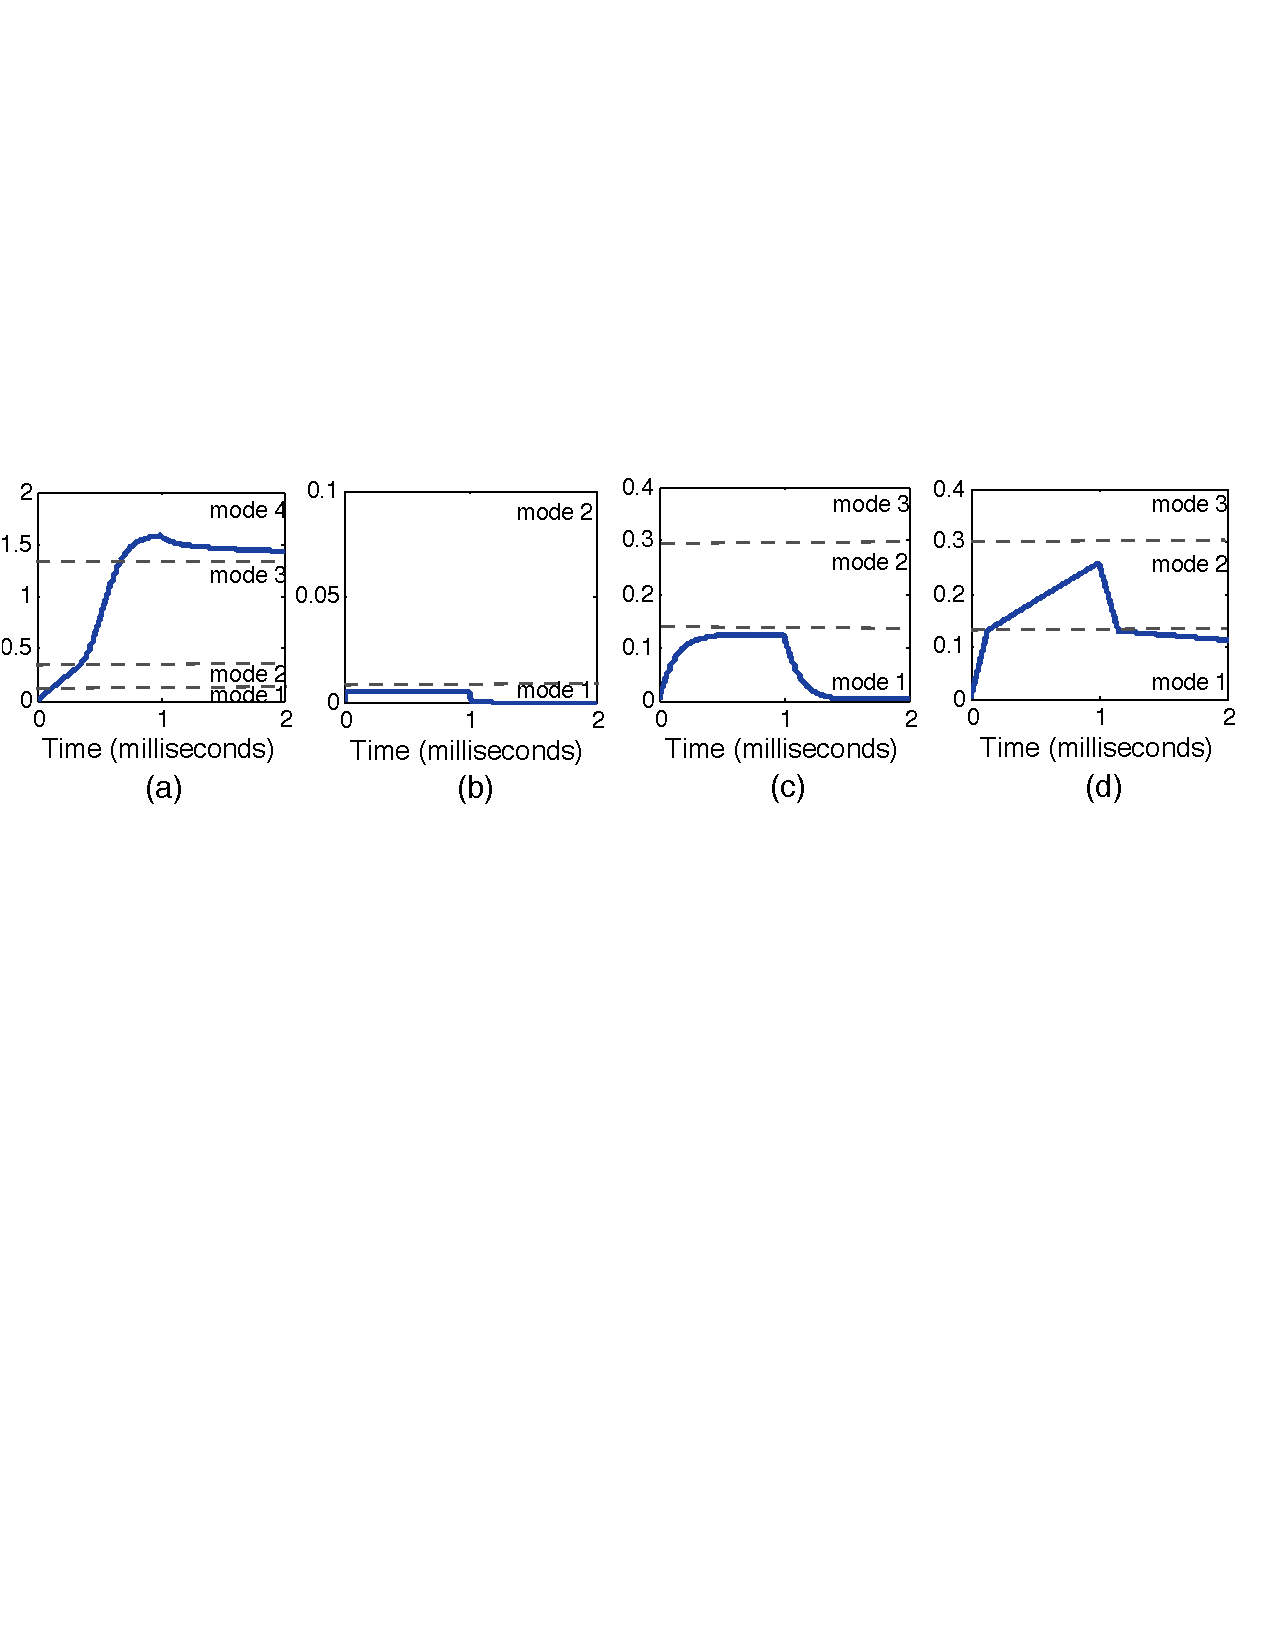
\includegraphics[scale=0.6]{fig-cardiactraj2}
\caption{Simulation results using disease related parameter values. (a) Original parameters (b) $\tau_{o1}=0.0055$ (c) $\tau_{o2} = 0.125$ (d) $\tau_{so1} =1.2$, $\tau_{so2} =1.0$ }
\label{cresults}
 %\vspace{-0.7cm}
\end{figure}

%%% Local Variables:
%%% TeX-master: "main"
%%% End:
